
\section{Anexo A: Integración de un Sensor de Espectro Radioeléctrico en la Plataforma IIoT}

Como parte del proceso de fortalecimiento de capacidades técnicas en la plataforma de entrenamiento IIoT, se integró dentro de la estación de radioastronomía CASIRI un dispositivo de monitoreo del espectro radioeléctrico destinado a la supervisión del entorno electromagnético. Esta integración tiene como finalidad complementar los datos industriales de CASIRI con información del comportamiento espectral del entorno, permitiendo identificar interferencias, disponibilidad de canal, congestión espectral u otros eventos relevantes para la transmisión inalámbrica de datos en contextos industriales.

\subsection{Características del Dispositivo Espectrómetro}
El dispositivo de monitoreo está diseñado para realizar adquisiciones precisas en ubicaciones fijas, y sus mediciones están georreferenciadas mediante los siguientes parámetros:
\begin{itemize}
    \item \textbf{Latitud y longitud:} Posición geográfica exacta.

    \item \textbf{Azimut:} Orientación horizontal de la antena receptora.

    \item \textbf{Elevación:} Ángulo vertical respecto al horizonte.

    \item \textbf{Altitud:} Altura sobre el nivel del mar o sobre el terreno de referencia.

\end{itemize}

Estas variables permiten una trazabilidad completa del entorno espectral observado y son registradas junto con la medición en cada adquisición.

\subsection{Actualización de la Arquitectura Método Parris}
La integración del espectrómetro implicó una actualización en la arquitectura del método Parris implementado en la plataforma. Se añadió un nuevo nodo de adquisición que publica los datos del espectro al broker MQTT bajo una estructura de tópicos adicional, en coherencia con el modelo jerárquico del método como se muestra a continuación.

\begin{center}
    UNS Path 4: \textit{UIS\_Central/Radiogis\_Casiri\_Sensor Espectro/<device\_id>}
\end{center}

Esta integración se diseñó considerando dos modos de operación:

\textbf{Modo On-line:} El espectrómetro transmite los datos directamente al broker MQTT mediante un cliente publicador. Esta opción permite la disponibilidad en tiempo real de los datos espectrales en la plataforma Ignition de nivel Enterprise, donde pueden ser procesados, visualizados y almacenados.

\textbf{Modo Off-line:} En escenarios donde no se cuenta con conectividad a internet, se activa un mecanismo de contingencia. El espectrómetro transmite los datos a un webservice receptor local que transforma las mediciones en archivos .txt o .json. Esta solución funciona como una base de datos local temporal. Una vez restablecida la conectividad, un webservice transmisor se encarga de sincronizar los datos acumulados hacia el servidor central de Ignition, asegurando que no se pierda ninguna adquisición.

\begin{figure}[H]
\centerline{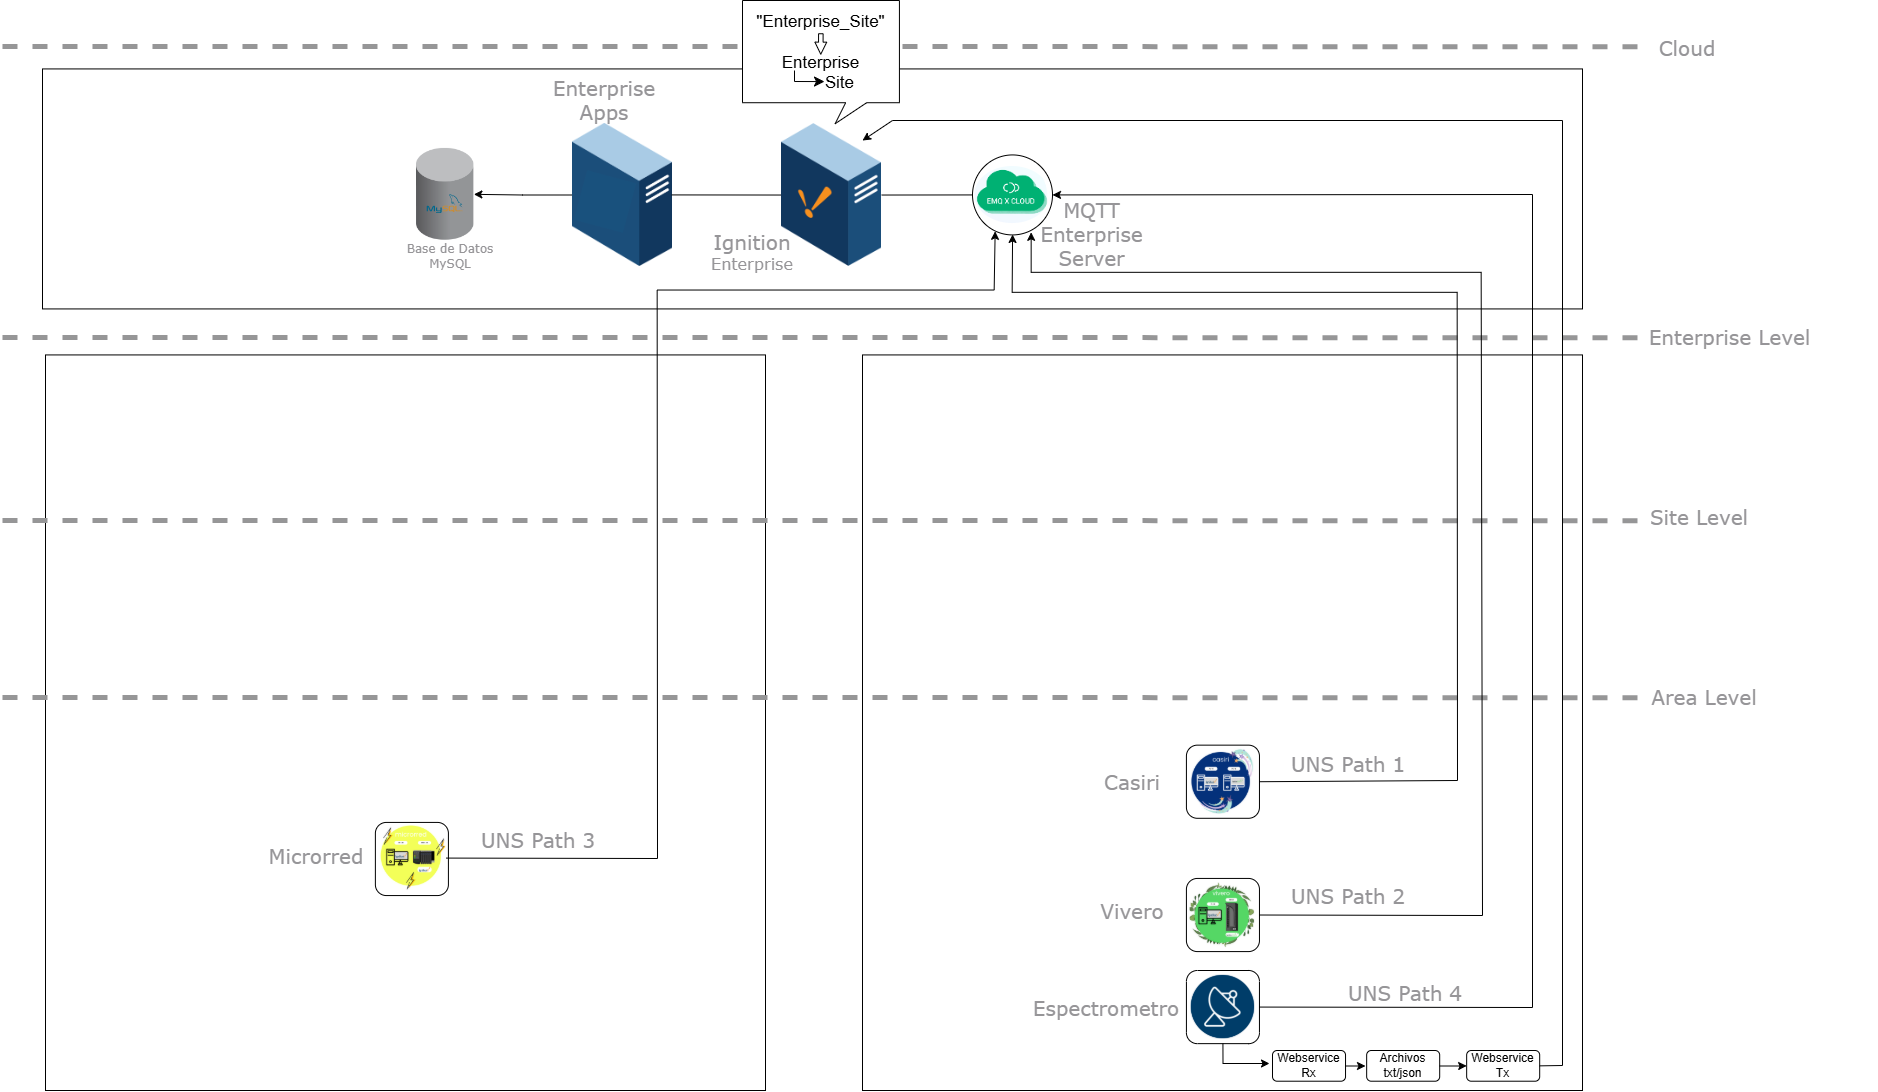
\includegraphics[width=19cm]{Figuras/ArqParris_IIoT_V4.png}}
\caption{Esquema de la Arquitectura UNS con el Metodo de Parris integrado el Espectrometro}
\label{fig:arqIIoT_Parris_V2}
\end{figure}


Un \textit{Webservice} es un servicio web que permite la comunicación y el intercambio de datos entre diferentes aplicaciones o sistemas a través de internet o redes locales, utilizando protocolos estándar como HTTP. Funciona mediante solicitudes y respuestas: una aplicación cliente envía una solicitud al servidor que ofrece el servicio, y este responde con la información solicitada o ejecuta una acción determinada. Los datos intercambiados generalmente se estructuran en formatos TXT o JSON, lo que facilita su interpretación por distintos lenguajes de programación. En este contexto, en la arquitectura de la Fig. \ref{fig:arqIIoT_Parris_V2} el webservice actúa como un puente entre el dispositivo que genera los datos (el espectrómetro) y el servidor que los recibe, permitiendo una transferencia segura incluso en entornos distribuidos permitiendo que los datos críticos del espectro no se pierdan aún en condiciones de red adversas.

\subsection{Visualización del Espectro en Ignition}
Con el objetivo de brindar una interfaz accesible para los operadores y usuarios de la plataforma, se añadió una nueva vista en la aplicación desarrollada en Ignition. Esta nueva vista muestra el espectro medido en tiempo real o histórico, (dependiendo de la disponibilidad de conexión a internet y del origen de los datos) y sus parámetros de adquisición.

\begin{figure}[H]
\centerline{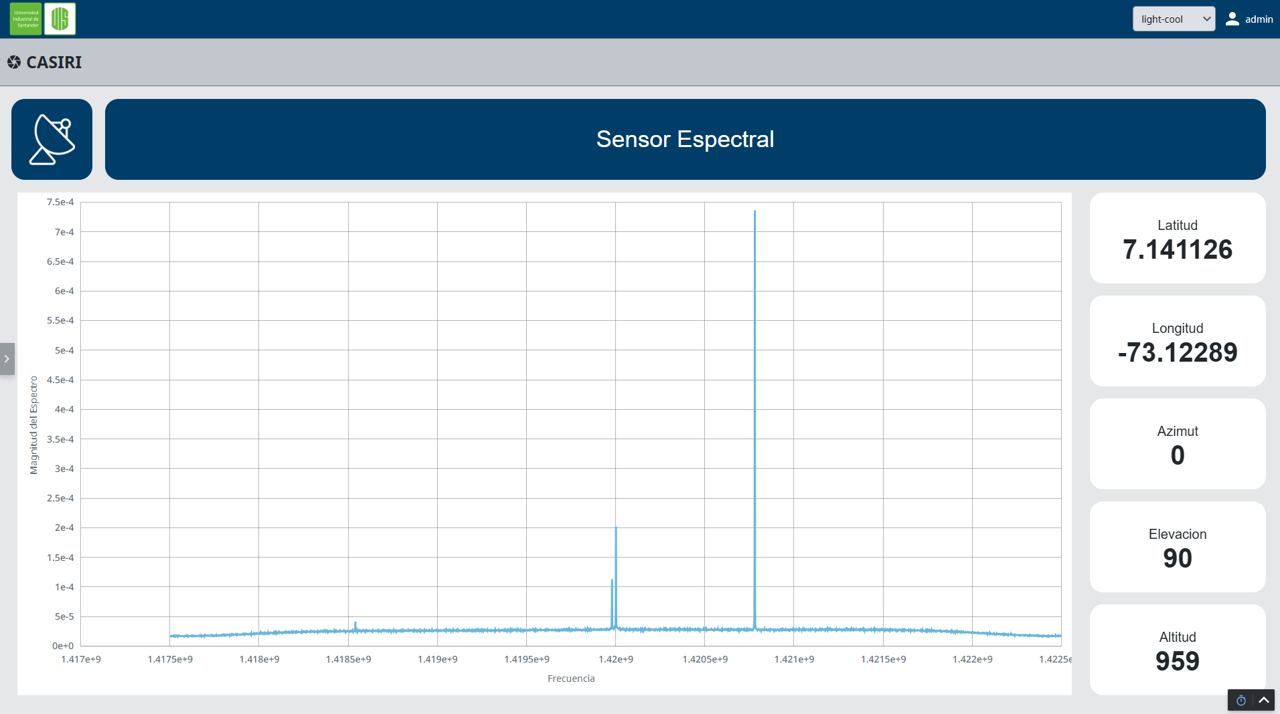
\includegraphics[width=14.1cm]{Figuras/Ig_Espectro}}
\caption{Vista de Espectrómetro de Casiri en la aplicación de Ignition}
\label{fig:espectroView}
\end{figure}

Los usuarios pueden consultar espectros correspondientes a ubicaciones específicas, visualizar el comportamiento en diferentes bandas de frecuencia y acceder a la información almacenada en diferentes tiempos. Esto amplía la capacidad de análisis de la plataforma, integrando no solo variables del proceso, sino también condiciones del entorno de comunicación inalámbrica.

\subsection{Consideraciones Finales}
La incorporación del sensor de espectro radioeléctrico fortalece la plataforma IIoT al ampliar el alcance de las variables monitoreadas por Casiri y permitir una evaluación más integral del entorno operativo. Desde la perspectiva del Unified Namespace, esta integración demuestra la flexibilidad del modelo para incorporar nuevos tipos de datos y adaptarse a condiciones variables de conectividad.

La arquitectura propuesta combina la jerarquía estructurada del método Parris con un enfoque práctico para la tolerancia a fallos, lo que refuerza su aplicabilidad en entornos industriales reales donde las condiciones de red no siempre son ideales.



